\subsection{Update step}
\label{subsec:toro_update}
The update equation of the EKF is given in Equation \ref{eq:ekf_correct}. The measurement equation of the system is given by $$\hat{y}_{k+1} = h(\hat{x}_{k+1}^-,u_{k+1},0).$$ For the sake of simplicity let us assume the measurement of noise uncorrelated. That is the noise acting on a measurement does not depend on the noise acting on all other measurements. $$V_k = I_3.$$ Substituting the assumption in Equation \ref{eq:ekf_correct} gives
\begin{equation}
\label{eq:correct}
\begin{split}
K_{k+1} &= P_{k+1}^-\hat{C}_{k+1}^{T-}(\hat{C}_{k+1}^-P_{k+1}^-\hat{C}_{k+1}^{T-} + R_{k+1})^{-1}\\
\hat{x}_{k+1} &= \hat{x}_{k+1}^- + K_{k+1}(y_{k+1}-\hat{y}_{k+1})\\
P_{k+1} &= (I- K_{k+1}\hat{C}_{k+1}^-)P_{k+1}^-.
\end{split}
\end{equation}
The measurements of \emph{Toro} are Cartesian accelerations($acc^b$) of the hip measured by accelerometer, angular velocity($\omega^b$) of the hip measured by the gyroscope, joint angles($q_j$) and joint velocities($\dot{q_j}$) measured by joint encoders.
\begin{equation}
    \label{eq:y_sens}
     y_{sens} = \begin{bmatrix} acc^b \\ \omega^b \\ q_j \\ \dot{q}_j \end{bmatrix} 
\end{equation}
\begin{itemize}
    \item The simplified model of $IMU_{acc}$ is $$ acc^b= \begin{bmatrix} acc^b_x \\ acc^b_y \\ acc^b_z \end{bmatrix} =  \begin{bmatrix}\ddot{p}_x^b \\ \ddot{p}_y^b \\ \ddot{p}_z^b \end{bmatrix} - R^T \begin{bmatrix}0 \\0 \\-9.81 \end{bmatrix}$$ \emph{R} is the rotational matrix that transforms a vector in body coordinate frame to spatial frame.
    \item $\ddot{p}^b$ is computed from the forward dynamic equation \ref{eq:motion} using the predicted values of the state
    \item $\omega_{f}^{b} $ is the vector of angular rates of the hip(floating base) measured by gyroscope. The measurements are in the frame attached to the hip. 
\end{itemize}
\begin{figure}
    \begin{center}
    %trim option's parameter order: left bottom right top
    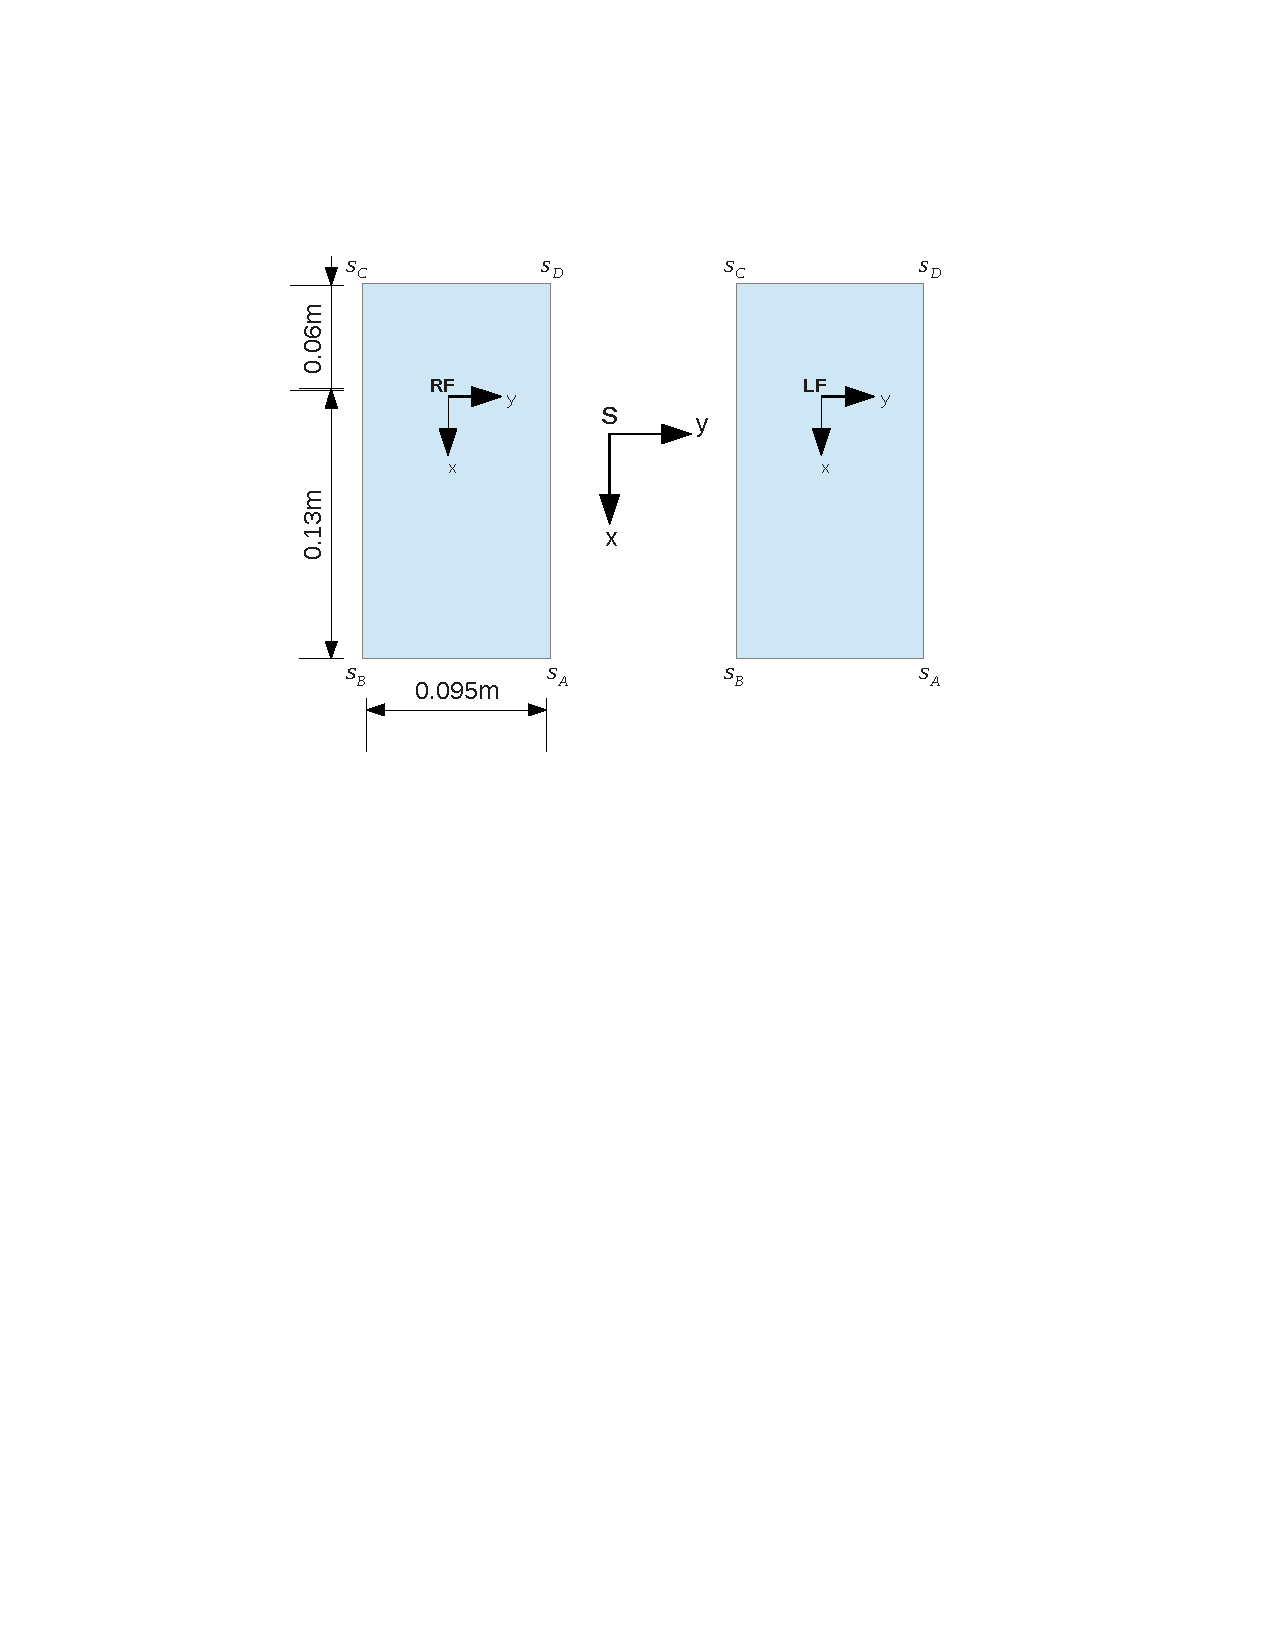
\includegraphics[trim= 20mm 150mm 20mm 50mm,scale=0.80]{Bilder/foot_topview.pdf}
    \caption{Toro feet viewed from top}
    \label{fig:biped_feet}
    \end{center}
\end{figure}
Along with the sensor measurements kinematic constraints can also be introduced as measurements \citep{atk12}. The kinematic constraint that is considered as measurement is the position constraint. For instance when the robot is tilting around an edge, the position of the points that are lying on that edge does not change with respect to the spatial frame (world frame). 
 
 Figure \ref{fig:biped_feet} shows the contact points considered for measurements. The corner points of each foot are measured with respect to spatial frame \emph{S}. The measuremnt equation of these contact points are
\begin{equation}
    \label{eq:y_kin}
    \begin{split}
    y_{kin} &= s_{contact} = \begin{bmatrix}s_{r}\\ s_{l}\end{bmatrix},\\
    \end{split}
\end{equation} where
$s_{r},s_{l}$ are the vectors of contact points in right foot and left foot defined with respect to spatial frame. They are given as
\begin{equation}
    \begin{split}
    s_{r} &= \begin{bmatrix} s_{A,r}\\ s_{B,r}\\ s_{C,r}\\ s_{D,r}\end{bmatrix}= \begin{bmatrix} {H}_{r}s_{A}\\  {H}_{r}s_{B}\\  {H}_{r}s_{C}\\  {H}_{r}s_{D}\end{bmatrix} \\
    s_{l} &= \begin{bmatrix} s_{A,l}\\ s_{B,l}\\ s_{C,l}\\ s_{D,l}\end{bmatrix}= \begin{bmatrix} {H}_{l}s_{A}\\  {H}_{l}s_{B}\\  {H}_{l}s_{C}\\  {H}_{l}s_{D}\end{bmatrix} \\
    \end{split}
\end{equation}
where ${H}_{r},{H}_{l}$ are the homogeneous transformation matrices of the right and left foot with respect to spatial frame [Appendix \ref{sec:htm}]
 In Figure \ref{fig:biped_feet} $s_A,s_B,s_C,s_D$ are constant with resptect to the foot coordinate frames \emph{RF,LF}. They are given as 
 $$ s_A = \begin{bmatrix} 0.13 \\ 0.0475 \\ 0 \end{bmatrix} , 
    s_B = \begin{bmatrix} 0.13 \\ -0.0475 \\ 0 \end{bmatrix},
    s_C = \begin{bmatrix} -0.06 \\ -0.0475 \\ 0 \end{bmatrix} \text{ and }
    s_D = \begin{bmatrix} -0.06 \\ 0.0475 \\ 0 \end{bmatrix}.$$

\paragraph{Switching:} The measurement of the contact points with respect to the spatial frame \emph{S} are made before starting the experiment. The measurements are made under the circumstance where both feet of the robot is in contact with the ground. These measurements are assumed to remain constant throughout the experiment. When the robot is standing on the ground, all the contact measurements are valid. But when the robot starts to tilt around an edge, some of the point measurements becomes invalid. For instance let us consider standing on right leg, when the robot is tilting around the back edge, the points $s_{C}$ and $s_{D}$ remain in contact with the ground, whereas the points $s_{A}$ and $s_B$ lifts off from the floor. The measurements from these points are not valid. It is important to detect the situations when the robot is standing still and when it is tilting around an edge, so that we consider only the valid measurements. Zero moment point (ZMP) is an useful criteria for detecting the tilting edge. The ZMP of a foot is computed from the ground reaction force measured by the FTS [Appendix \ref{sec:zmp}]. The contact measurements also differ when the a single foot is in contact (single support) or two feet are in contact(double support). The single and double support cases can be differentiate by measuring the vertical ground reactional force $F_z$. The contact case is determined by the parameter $\alpha$ which is given as \citep{atk12} $$ \alpha = \frac{F_{z,r} + F_{z,l}}{F_{z,r}}.$$ 

\begin{algorithm}
    \caption{Selection of contact measurements}
    \label{alg:cnt_switch}
    \begin{algorithmic}
    %\REQUIRE  $s_{cnt}$
    %\ENSURE $FOO$
    \IF {$\alpha = 0.5$}
    %{Double support}
        \IF {$ {zmp}_x \geq 0.12$}
        % Tilting around front edge
        \RETURN $ s_{cnt}= \begin{bmatrix}s_{A,r} &s_{B,r} &s_{A,l} &s_{B,l} \end{bmatrix}^T$ 
        \ELSIF {${zmp}_x \leq -0.05$}
        % Tilting around back edge
        \RETURN $ s_{cnt}= \begin{bmatrix}s_{C,r} &s_{D,r} &s_{C,l} &s_{D,l} \end{bmatrix}^T$ 
        \ENDIF
    \ELSIF {$\alpha = 1$}
    % Support right foot
        \IF {$ {zmp}_x \geq 0.12$}
        % Tilting around front edge
        \RETURN $ s_{cnt}= \begin{bmatrix}s_{A,r} &s_{B,r}  \end{bmatrix}^T$ 
        \ELSIF {${zmp}_x \leq -0.05$}
        % Tilting around back edge
        \RETURN $ s_{cnt}= \begin{bmatrix}s_{C,r} &s_{D,r}  \end{bmatrix}^T$ 
        \ELSIF {$ {zmp}_y \geq 0.04$}
        % Tilting around inner edege
        \RETURN $ s_{cnt}= \begin{bmatrix}s_{A,r} &s_{D,r}  \end{bmatrix}^T$ 
        \ELSIF {${zmp}_y \leq -0.04$}
        % Tilting around outer edge
        \RETURN $ s_{cnt}= \begin{bmatrix}s_{B,r} &s_{C,r}  \end{bmatrix}^T$ 
        \ENDIF
    \ELSIF {$\alpha = 0$}
    % Support left foot
        \IF {$ {zmp}_x \geq 0.12$}
        % Tilting around front edge
        \RETURN $ s_{cnt}= \begin{bmatrix} s_{A,l} &s_{B,l} \end{bmatrix}^T$ 
        \ELSIF {${zmp}_x \leq -0.05$}
        % Tilting around back edge
        \RETURN $ s_{cnt}= \begin{bmatrix} s_{C,l} &s_{D,l} \end{bmatrix}^T$ 
        \ELSIF {$ {zmp}_y \geq 0.04$}
        % Tilting around outer edege
        \RETURN $ s_{cnt}= \begin{bmatrix}s_{A,r} &s_{D,r}  \end{bmatrix}^T$ 
        \ELSIF {${zmp}_y \leq -0.04$}
        % Tilting around inner edge
        \RETURN $ s_{cnt}= \begin{bmatrix}s_{B,r} &s_{C,r}  \end{bmatrix}^T$ 
        \ENDIF
    \ENDIF
    \end{algorithmic}
\end{algorithm}

The Algorithm \ref{alg:cnt_switch} is useful in making the decision about the contact points $s_{cnt}$ based on number of support and ZMP. The ZMP is defined with respect to the foot coordinate frame. For instance the front edge of right foot in Figure \ref{fig:biped_feet} is $0.13m$ from the foot coordinate frame $RL$. When the ${zmp}_x$ of the foot reaches this value then the foot starts to tilt around the front edge. Like wise the foot starts tilting backwards when the ${zmp}_x$ reaches the value $-0.06$. Likewise the upper and lower bounds of $zmp_y$ are $0.0475$ and $-0.0475$.

The full measurement equations of the system is obtained by combining Equations \ref{eq:y_sens} and \ref{eq:y_kin}. The discretized form of measurement equations is
\begin{equation}
    \label{eq:y_msr}
    y_{k+1} = \begin{bmatrix} y_{sens,k+1} \\ y_{kin,k+1} \end{bmatrix}= \begin{bmatrix} acc^b_{k+1} \\ \omega^b_{k+1} \\ q_{k+1} \\ \dot q_{k+1} \\ s_{cnt,k+1} \end{bmatrix}.
\end{equation}

For the computation of Kalman gain $K_k$ and to update the error covariance matrix $P_k$ in Equation \ref{eq:correct}, the measurement sensitivity matrix $C_k$ have to be computed. The matrix $C_k$ determined by computing the Jacobian matrix of the measurement equation \ref{eq:y_msr}. The computation of $C_k$ matrix is as follows:
\begin{enumerate}
\item The measurement equation for acceleration measurements is  $$\hat{acc}^b_{k+1} = \dot{v}^{b-}_{k+1}-\hat{R}_{k+1}^{T-}\begin{bmatrix} 0 \\ 0 \\ -9,81 \end{bmatrix}$$.
The Jacobian matrix is 
\begin{equation}
    \label{eq:dacc_msrdx}
    \dfdx{\hat{acc}_{k+1}^{b-}}{x} = \dfdx{\hat{\dot{v}}_{k+1}^{b-}}{x} - \dfdx{\hat{R}^{T-}_{k+1}}{x}\begin{bmatrix} 0 \\ 0 \\ -9,81 \end{bmatrix}  \in \Re^{3 \times 62}
\end{equation}where
\begin{itemize}
    \item $\dfdx{\hat{\dot{v}}_{k+1}^b}{x}$ is Jacobian matrix obtained by evaluating Equation \ref{eq:dydx} with the values $\hat x_{k+1}^-, u_{k+1}$ and picking the rows corresponding to the linear acceleration. For instance in Equation \ref{eq:dydx} the first three rows of the Jacobian matrix corresponds to the linear acceleration.
    \item $\dfdx{\hat{R}^T_{k+1}}{x}$ is partial derivative of Rotation matrix [Appendix \ref{sec:rot_mat}].
\end{itemize}

\item The Jacobian matrix corresponding to the angular velocity $\hat{\omega}^{b-}_{k+1}$ is 
\begin{equation}
    \label{eq:dw_msrdx} 
    \dfdx{\hat{\omega}^{b-}_{k+1}}{x} = \left(\dfdx{\hat{\omega}^{b-}_{k+1}}{x_{1}}, \dfdx{\hat{\omega}^{b-}_{k+1}}{x_{2}}, \cdots , \dfdx{\hat{\omega}^{b-}_{k+1}}{x_{62}}\right) \in \Re^{3 \times 62}
\end{equation}
\[ \dfdx{\hat{\omega}^{b-}_{k+1}}{x} = 
    \begin{cases}
    l_{3,i-34} & \text{if } 34 < i \leq 37 \\
    \textbf{0}_{3,1} &\text{otherwise}.
    \end{cases}
 \]where 
 \begin{itemize}  
 \item $l_{x,y}$ is a zero vector of length $x$ with 1 at the $y^{th}$ position.
 \item $\textbf{0}_{m,n}$ is the zero matrix of dimensions $m$ and $n$.
 \end{itemize}

\item The Jacobian matrix corresponding to the joint angles $\hat{q}_{k+1}^-$ is
\begin{equation}
\label{eq:dq_msrdx}
\dfdx{\hat{q}_{k+1}^-}{x} = \left(\dfdx{\hat{q}_{k+1}^-}{x_{1}}, \dfdx{\hat{q}_{k+1}^-}{x_{2}}, \cdots , \dfdx{\hat{q}_{k+1}^-}{x_{62}}\right) \in \Re^{25 \times 62}
\end{equation}
 \[
 \dfdx{\hat{q}_{k+1}^-}{x_{i}} =
 \begin{cases}
 l_{25,i-6} & \text{if } 6 < i \leq 31 \\
 \textbf{0}_{25,1} & \text{otherwise}.
 \end{cases}
 \]

\item The Jacobian matrix corresponding to the angular velocity of joint angles  $\hat{\dot{q}}_{k+1}^-$ is 
\begin{equation}
 \label{eq:ddq_msrdx}
\dfdx{\hat{\dot{q}}_{k+1}^-}{x} = \left(\dfdx{\hat{\dot{q}}_{k+1}^-}{x_{1}}, \dfdx{\hat{\dot{q}}_{k+1}^-}{x_{2}}, \cdots , \dfdx{\hat{\dot{q}}_{k+1}^-}{x_{62}}\right) \in \Re^{25 \times 62}
\end{equation}
  \[
 \dfdx{\hat{\dot{q}}_{k+1}^-}{x_{i}} =
 \begin{cases}
 l_{25,i-37} & \text{if } 37 < i \leq 62 \\
 \textbf{0}_{25,1} & \text{otherwise}.
 \end{cases}
 \]

 \item The measurement equation for the contact points in right and left foot are 
 $$ \hat{s}_{cnt,k+1}=
 \begin{bmatrix}
 \hat{s}_{r,k+1}^- \\ \hat{s}_{l,k+1}^-
 \end{bmatrix} 
 = \begin{bmatrix}
 \hat{H}_{r,k+1}^- s  \\ \hat{H}_{l,k+1}^- s
   \end{bmatrix}
	$$ 
where $s$ can be zero or more points in the set $ \lbrace s_A,s_B,s_C,s_D \rbrace$. The points in contact $s$ is determined by the Algorithm \ref{alg:cnt_switch}. 

 The Jacobian matrix of the contact measurements is 
\begin{equation}
    \label{eq:dscnt_msrdx}
    \begin{split}
    \dfdx{\hat{s}_{cnt,k+1}^-}{x} &= \left[
    \begin{aligned}
    \dfdx{\hat{s}_{r,k+1}^-}{x}  \\ \dfdx{\hat{s}_{l,k+1}^-}{x}
    \end{aligned} \right] = \left[
    \begin{aligned}
    \dfdx{\hat{H}_{r,k+1}^-}{x}s \\ \dfdx{\hat{H}_{l,k+1}^-}{x}s 
    \end{aligned}\right]
 \\ \vspace{5mm} \\
     \dfdx{\hat{H}_{f,k+1}^-}{x} = &\left( \dfdx{\hat{H}_{f,k+1}^-}{x_1}, \dfdx{\hat{H}_{f,k+1}^-}{x_2},\cdots, \dfdx{\hat{H}_{f,k+1}^-}{x_{62}} \right) \hspace{5mm} f \in \{r,l\}
     \end{split}
\end{equation}
where $\dfdx{\hat{H}_{f,k+1}^-}{x}$ is the partial derivative of homogeneous transformation matrix of a foot with respect to the system states [Appendix \ref{sec:htm}].
\end{enumerate}
The measurement sensitivity matrix $\hat{C}_{k+1}^-$ of the system is given by Equations \ref{eq:dacc_msrdx}, \ref{eq:dw_msrdx}, \ref{eq:dq_msrdx}, \ref{eq:ddq_msrdx}and \ref{eq:dscnt_msrdx}:
\begin{equation}
    \label{eq:msr_mat}
    \hat{C}^-_{k+1} = \left(
   \begin{aligned}
   \dfdx{\hat{acc}_{k+1}^{b-}}{x} \\
   \dfdx{\hat{\omega}^{b-}_{k+1}}{x} \\
    \dfdx{\hat{q}_{k+1}^-}{x} \\
    \dfdx{\hat{\dot{q}}_{k+1}^-}{x} \\
    \dfdx{\hat{s}_{cnt,k+1}^-}{x} \\
   \end{aligned}
	 \right) \in \Re^{80 \times 62}.
\end{equation}

\begin{comment}
\paragraph{Observability:}
State space representation of a linear system is,
\begin{equation}
\label{eq:dyn_l}
\begin{split}
\dot{x} &= Ax + Bu\\
y &= Cx + Du.
\end{split}
\end{equation}
where, $x \in \Re^{n}$ is the vector representing the states of the system. $u \in \Re^{p}$ is the vector of inputs, $y \in \Re^{m}$ is the vector of outputs of the system. $A \in \Re^{n \times n}$ is the system matrix. $B \in \Re^{n \times p}$ is the matrix relating state and input, $C \in \Re^{m \times n}$ is the measurement matrix relating output and state, $D \in \Re^{m \times p}$ is the matrix relating input and output of the system.

Linearising a nonlinear system in Equation \ref{eqn:nl_sys} at some operating point will lead to linear system of form Eq. \ref{eq:dyn_l}. For a linear system to be observable, it should satisfy
\begin{equation}
obs =
\begin{pmatrix}
C\\ CA \\ CA^{2}\\ \vdots \\ CA^{n-1}
\end{pmatrix}
, rank(obs) =n
\end{equation}
For our system to be observable $rank(obs) = 62$.
\end{comment}
%\textbf{ Make plots from files act=datsrc/ROBOT-TILT-0807.mat est=estimates-data/est-090701.mat or *080703.mat }
%\end{document}
